\documentclass[10pt]{beamer}
%\usepackage[fontset=none]{ctex}
\usepackage{graphicx}
\usepackage{listings}
\usepackage{ulem}
\usepackage{boxedminipage}
% Copyright 2007 by Till Tantau
%
% This file may be distributed and/or modified
%
% 1. under the LaTeX Project Public License and/or
% 2. under the GNU Public License.
%
% See the file doc/licenses/LICENSE for more details.


% Common packages

%\usepackage{babel}
%\usepackage[latin1]{inputenc}
\usepackage{times}
\mode<article>
{
  \usepackage{times}
  \usepackage{mathptmx}
  \usepackage[left=1.5cm,right=6cm,top=1.5cm,bottom=3cm]{geometry}
}

\usepackage{hyperref}
%\usepackage[T1]{fontenc}
%\usepackage{tikz}
%\usepackage{colortbl}
%\usepackage{translator} % comment this, if not available


% Common settings for all lectures in this course

\def\lecturename{}

\title{\insertlecture}

\author{}

\institute
{
    Fang Yuan (yfang@nju.edu.cn)\\
  School of Electronics Science and Engineering\\
  Nanjing University
}

\subject{\lecturename}


% Beamer version theme settings

\useoutertheme[height=0pt,width=2cm,right]{sidebar}
\usecolortheme{rose,sidebartab}
\useinnertheme{circles}
\usefonttheme[only large]{structurebold}

\setbeamercolor{sidebar right}{bg=black!15}
\setbeamercolor{structure}{fg=blue}
\setbeamercolor{author}{parent=structure}

\setbeamerfont{title}{series=\normalfont,size=\LARGE}
\setbeamerfont{title in sidebar}{series=\bfseries}
\setbeamerfont{author in sidebar}{series=\bfseries}
\setbeamerfont*{item}{series=}
\setbeamerfont{frametitle}{size=}
\setbeamerfont{block title}{size=\small}
\setbeamerfont{subtitle}{size=\normalsize,series=\normalfont}

\setbeamertemplate{navigation symbols}{}
\setbeamertemplate{bibliography item}[book]
\setbeamertemplate{sidebar right}
{
  {\usebeamerfont{title in sidebar}%
%    \vskip1.5em%
    \hskip3pt%
    \usebeamercolor[fg]{title in sidebar}%
%    \insertshorttitle[width=2cm,center,nolinebreaks]\par%
    \vskip1.25em%
  }%
  {%
    \hskip3pt%
    \usebeamercolor[fg]{author in sidebar}%
    \usebeamerfont{author in sidebar}%
    \insertshortauthor[width=1cm,center,respectlinebreaks]\par%
 %   \vskip1.25em%
  }%
  \hbox to2cm{\hss\insertlogo\hss}
  \vskip1.25em%
  \insertverticalnavigation{2cm}%
  \vfill
  \hbox to 2cm{\hfill\usebeamerfont{subsection in
      sidebar}\strut\usebeamercolor[fg]{subsection in
      sidebar}\insertshortlecture.\insertframenumber\hskip5pt}%
  \vskip3pt%
}%

\setbeamertemplate{title page}
{
  \vbox{}
  \vskip2cm
  {\usebeamercolor[fg]{title}\usebeamerfont{title}\inserttitle\par}%
  \ifx\insertsubtitle\@empty%
  \else%
    \vskip0.25em%
    {\usebeamerfont{subtitle}\usebeamercolor[fg]{subtitle}\insertsubtitle\par}%
  \fi%     
  \vskip1em\par
%  Lecture \emph{\lecturename}\ , \insertdate\par
  \vskip0pt plus1filll
  \leftskip=0pt plus1fill\insertauthor\par
  \insertinstitute\vskip1em
}

\logo{
\includegraphics[width=1cm]{njulogo.pdf}}


% Article version layout settings

\mode<article>

\makeatletter
\def\@listI{\leftmargin\leftmargini
  \parsep 0pt
  \topsep 5\p@   \@plus3\p@ \@minus5\p@
  \itemsep0pt}
\let\@listi=\@listI


\setbeamertemplate{frametitle}{\paragraph*{\insertframetitle\
    \ \small\insertframesubtitle}\ \par
}
\setbeamertemplate{frame end}{%
  \marginpar{\scriptsize\hbox to 2cm{\sffamily%
      \hfill\strut\insertshortlecture.\insertframenumber}\hrule height .2pt}}
\setlength{\marginparwidth}{1cm}
\setlength{\marginparsep}{4.5cm}

\def\@maketitle{\makechapter}

\def\makechapter{
  \newpage
  \null
  \vskip 2em%
  {%
    \parindent=0pt
    \raggedright
    \sffamily
    \vskip8pt
    {\fontsize{36pt}{36pt}\selectfont \insertshortlecture \par\vskip2pt}
    {\fontsize{24pt}{28pt}\selectfont \color{blue!50!black} \insertlecture\par\vskip4pt}
    {\Large\selectfont \color{blue!50!black} \insertsubtitle\par}
    \vskip10pt

    \normalsize\selectfont \@date\par\vskip1.5em
    \hfill Fang Yuan, ESE, NJU
  }
  \par
  \vskip 1.5em%
}

\let\origstartsection=\@startsection
\def\@startsection#1#2#3#4#5#6{%
  \origstartsection{#1}{#2}{#3}{#4}{#5}{#6\normalfont\sffamily\color{blue!50!black}\selectfont}}

\makeatother

\mode
<all>


% New useful definitions:

\newbox\mytempbox
\newdimen\mytempdimen

\newcommand\includegraphicscopyright[3][]{%
  \leavevmode\vbox{\vskip3pt\raggedright\setbox\mytempbox=\hbox{\includegraphics[#1]{#2}}%
    \mytempdimen=\wd\mytempbox\box\mytempbox\par\vskip1pt%
    \fontsize{3}{3.5}\selectfont{\color{black!25}{\vbox{\hsize=\mytempdimen#3}}}\vskip3pt%
}}

\newenvironment{colortabular}[1]{\medskip\rowcolors[]{1}{blue!20}{blue!10}\tabular{#1}\rowcolor{blue!40}}{\endtabular\medskip}

\def\equad{\leavevmode\hbox{}\quad}

\newenvironment{greencolortabular}[1]
{\medskip\rowcolors[]{1}{green!50!black!20}{green!50!black!10}%
  \tabular{#1}\rowcolor{green!50!black!40}}%
{\endtabular\medskip}



\lecture[1]{A short introduction to \LaTeX\\[5ex]
  $\tau \epsilon \chi$ (technology $\to$ TeX)}{}

\begin{document}
\begin{frame}
  \maketitle
\end{frame}

\begin{frame}\frametitle<presentation>{Contents}
  \tableofcontents

   \url{https://github.com/yfang1644/tex_intro}
\end{frame}

\section{What is \LaTeX}
\begin{frame}{What is \TeX}
\begin{itemize}
    \item \TeX{} is a typesetting system (or {\em formatting system})
    that allows you to produce high-quality printable documents.

    \item \TeX{} was written by Donald Knuth, released in 1978,
    when he wrote his book \alert{The Art of Computer Programming}.
\end{itemize}
\begin{center}
    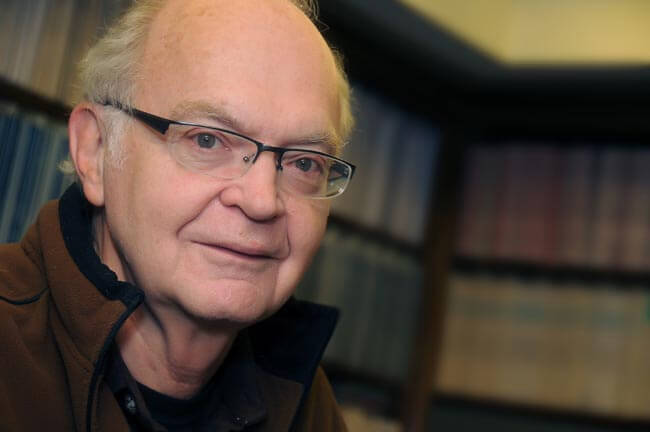
\includegraphics[width=.55\textwidth]{Donald-Knuth.jpg}
\end{center}
    Donald Knuth(Jan. 10, 1938--): Turing Award(1974),
    National Academy of Sciences(1975) and many other awards and honors.
\end{frame}

\begin{frame}{What is \LaTeX}
\begin{itemize}
    \item \TeX{} system is too primitive. Leslie Lamport developed a document
    preparation system based on \TeX{} (1984).

\item \LaTeX{} is short for \alert{La}mport \alert{TeX{}}.
\end{itemize}
\begin{center}
    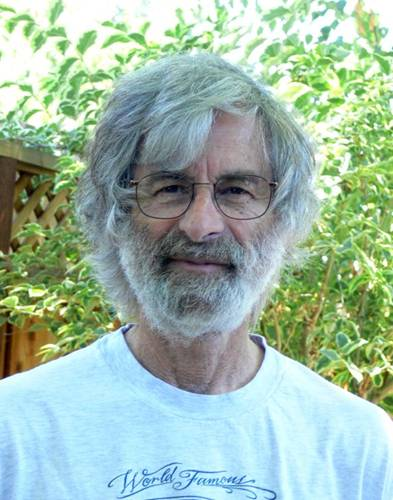
\includegraphics[width=.4\textwidth]{Leslie-Lamport.jpg}
\end{center}
    Leslie Lamport (Feb. 7, 1941--),
    John von Neumann Medal (2008),
    Turing Award(2013), ACM Fellow(2014), and more.
\end{frame}

\begin{frame}[t]{How a Book is Printed}
Imagine an author is publishing a book:
\begin{itemize}
    \item He gives his manuscript to a publishing company.
    \item A book designer, or an editor (of the company) chooses
        the document layout, page size, fonts, headings, ...,etc.
        He marks his instructions into the manuscript, then gives
        it to the typesetters.

        The editor needs knowledges both the author's and the publishing.
    \item The typesetters typeset the book according to these instructions.
\end{itemize}

    When you use WYSIWYG (\alert{What you see is what you get}),
    you pretend you are three of them.\\[10pt]

    When you use \TeX{}, you are just an author (you know little
    about publishing), \LaTeX{} is the editor, \TeX{} is typesetters

    But \LaTeX{} is only a program. You must give guidance, i.e.
    programming.
\end{frame}

\begin{frame}{Why Use \TeX{} And Why Not}
\LaTeX{} features:
\begin{itemize}
    \item Making beautiful and professional documents.
    \item Control over large documents containing sectioning,
        cross-references, tables and figures.
    \item Typesetting of complex mathematical formulas.
    \item Content lists, footnotes, indexes, ..., become very easy.
    \item Using plain text as opposed to the formatted text,
        makes the documents small, easy to edit and to maintain.
    \item Consistency.
    \item \TeX{} system is free of charge.
\end{itemize}

    But \TeX{} is not always the choice:
\begin{itemize}
    \item Very hard to write unstructured and disorganized documents
        (seminar presentations for example).
    \item Template designing takes a lot of time.
\end{itemize}
\end{frame}

\section{Beginners}
\begin{frame}{\TeX{} Source File}
\lstinputlisting[language={[LaTeX]TeX},
    morekeywords={maketitle},keywordstyle=\color{red}]{einstein.tex}
\end{frame}

\begin{frame}[t]{Commands and Environments}
    \LaTeX{} uses commands to format text.
\begin{itemize}
    \item A command starts with backslash and then have a name
        consisting of letters only.
    \item Some commands require parameters. Parameters are put in
        \{\ \ \} after command. Some commands take optional parameters.
        Optional parameter is put in [\ \ ].\\[2ex]

    \fbox{
        \textbackslash command[optional parameter]\{parameter\}\{parameter\}
    }
\end{itemize}

    Environments are special command using \textbackslash begin\{...\}
    and \textbackslash end\{...\}

\end{frame}

\begin{frame}[t]{\TeX{} Distributions}
\begin{table}
\centering
    \caption{\TeX{} distributions}
    \begin{tabular}{cc}\hline\hline
        OS          &   Distro\\\hline
        All-platform & TeX Live\\
        Windows    & MikTeX \\
        Mac OS    & MacTeX\\\hline\hline
    \end{tabular}
\end{table}

    We write \TeX{} document using text editor, and \alert{xelatex} to compile
    \TeX{} to produce PDF:\\[2ex]

\begin{center}
    \fbox{ \$ xelatex einstein.tex}
\end{center}

In IDE, this command is executed by clicking the compiling-icon.
\\[1ex]
Sometime, you need \alert{xelatex} twice or more to produce correct
cross-references.
\end{frame}

\begin{frame}{Learning Curve}
\begin{center}
    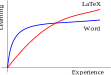
\includegraphics[width=0.4\textwidth]{learncurve.pdf}
\end{center}

\begin{itemize}
    \item 10 minutes of learning ``WORD'' may write a not-so-bad document.
    \item 1 -- 2 hours of learning \LaTeX{} can produce a not-so-bad
        PDF without too complex formulae, figures, and misc., almost
        no publishing mistakes.
    \item About 10 hours of learning \LaTeX{}, you can produce
        professional document with hundreds
        of pages, including content list, cross references,
        formulae, figures, tables, ...
\end{itemize}
\end{frame}

\section{Document Structure}
\begin{frame}[t]{Text}
    \TeX{} simple rules:
\begin{itemize}
    \item Input letters, digits and most ASCII chars as text, except only
        a few special symbols, which must be escaped
        (\alert{\textbackslash}).
    \item Multiple white spaces, tab stops are equal to one white space.
    \item Multiple blank lines are equal to one blank, which produce
        a paragraph separation.
\end{itemize}

    \alert{DO NOT} focus too much on {\em how the document looks like}.
    It is the publisher's job.

\end{frame}

\begin{frame}[t]{Sentence and Paragraph}
\begin{itemize}
    \item A group of text between blank lines forms a paragraph.
        A paragraph is the typographical form that should reflect
        one \alert{coherent} thought, or one idea.
    \item Words which put in a box are not broken by newline, i.e.
        \textbackslash mbox\{World-War-III\}.
    \item Command \alert{\textbackslash newline} or
        \alert{\textbackslash newpage} will change the form of

        a paragraph intentionally.
    \item Paragraphs should be structured logically at a higher level
        (\alert{subsection}, \alert{section}, \alert{chapter}, etc).
\end{itemize}
\end{frame}

\begin{frame}[t]{Document Structure}
Paragraphs are organized into sections.
A document is structured using following levels:
\begin{description}
    \item[-1] \textbackslash part\{...\}
    \item[0] \textbackslash chapter\{...\} (\alert{not used in article class})
    \item[1] \textbackslash section\{...\}
    \item[2] \textbackslash subsection\{...\}
    \item[3] \textbackslash subsubsection\{...\}
    \item[4] \textbackslash paragraph\{...\}
    \item[5] \textbackslash subparagraph\{...\}
\end{description}

Sections are automatically numbered. You should not number chapters
and sections intentionally. Besides, equations, theorems, figures,
tables, etc. are also numbered automatically.

    \fbox{\textbackslash setcounter\{tocdepth\}\{2\}}

    will list sections in content until level 2.
\end{frame}

\begin{frame}[t]{Big Projects}
    Big document can be split into several parts. \LaTeX{} uses
    command \alert{\textbackslash include} or \alert{\textbackslash input}
    to insert the contents of a file.\\[3ex]

\textbackslash title\{Civilizations\}

\textbackslash input Babylonian.tex \qquad \% Chapter 1

\textbackslash input Egypt.tex \qquad\qquad \% Chapter 2

\textbackslash input India.tex \qquad\qquad \% Chapter 3

\textbackslash input China.tex \qquad\qquad \% Chapter 4


\end{frame}

\begin{frame}[fragile]{Lists}
    \LaTeX{} uses 3 basic lists: itemize, enumerate and description.

\begin{verbatim}
Fibonacci function $fib(n)$:
\begin{enumerate}
    \item BEGIN
    \item if $n<2$ then return 1, goto \ref{end}
    \item calculate $fib(n-1)$ and $fib(n-2)$
    \item return $fib(n-1)+fib(n-2)$
    \item END \label{end}
\end{enumerate}
\end{verbatim}

\begin{boxedminipage}{0.8\textwidth}
    Fibonacci function $fib(n)$:
\begin{enumerate}
    \item BEGIN
    \item if $n<2$ then return 1, goto \ref{end}
    \item calculate $fib(n-1)$ and $fib(n-2)$
    \item return $fib(n-1)+fib(n-2)$
    \item END \label{end}
\end{enumerate}
    \end{boxedminipage}
\end{frame}

\section{Math Notation}
\begin{frame}{Math Mode}
    Inline and stand-alone math notations look different. Math symbols
    use different font from text.
\begin{itemize}
    \item Inline math mode between \$ and \$: $n!=\prod_{i=1}^n i$
    \item Stand-alone math mode between \$\$ and \$\$, or in
        \alert{equation} environment. Equation environment will
		automatically numbered.

		\begin{equation}\label{equ:xxx}
            \sum_{i=0}^n i = \frac{n (n-1)}{2} \nonumber
        \end{equation}
        \begin{equation}
            X(\omega) =\frac{1}{\sqrt{2\pi}} \int_{-\infty}^{\infty}
                x(t) e^{-j\omega t}\mathrm{d} t
        \end{equation}
    \item Greek letters: \textbackslash alpha, \textbackslash beta ,...
    \item Math symbols: \textbackslash int, \textbackslash sum,
        \textbackslash frac\{\}, \textbackslash lim,
        \textbackslash limits, \textbackslash nolimts,..., and more.

\end{itemize}
\end{frame}

\begin{frame}[t]{Newtheorem}

{\em Lemmas, Definitions, Axioms} and similar structures are often used
    in mathematical documents.\\[3ex]

    \fbox{
        \textbackslash newtheorem\{name\}[counter]\{text\}[section]}
    \\[3ex]

\alert{name} is a new environment name. \alert{text} is the text
printed in the document as a label. \alert{counter} specifies the
name of a previously declared {\em theorem}. \alert{section} specifies
the sectional unit within which the {\em theorem} should get its numbers.

    \begin{example}
        \textbackslash newtheorem\{law\}\{Law\}[section]
    \end{example}

\end{frame}

\begin{frame}[fragile]{Theorems}
\newtheorem{law}{Law}[section]
\begin{verbatim}
\begin{law}
  An object doesn't change its velocity
  unless acted upon by a force.
\end{law}
\begin{law}
  $$ \mathbf{F}=m\mathbf{a} $$
\end{law}
\end{verbatim}

will reads:

\begin{law}
  An object doesn't change its velocity unless acted upon by a force.
\end{law}
\begin{law}
  $$ \mathbf{F}=m\mathbf{a} $$
\end{law}

\end{frame}

\section{Figures and Tables}
\begin{frame}[fragile]{Figures and Tables}
    Figures and tables are called \alert{floating object}, because
    they occupy large space, i.e. they may not appear in the current
    context. Therefore, you should avoid using ``\sout{See figure below}''
    or ``\sout{Refer the table above}'' in your documents.

\begin{verbatim}
\begin{figure}
\centering
  \includegraphics[width=0.5\textwidth]{Knuth.jpg}
  \caption{Doland Knuth(1938--)}\label{pic:knuth}
\end{figure}
Fig.\ref{pic:knuth} is a photo of Doland Knuth.
\end{verbatim}

    \LaTeX{} supports both vector graphics(PDF, EPS) and raster graphics
    (JPG, PNG, BMP, etc.).

\end{frame}

\begin{frame}[fragile]{Figures and Tables}
\begin{verbatim}
\begin{table}
\centering \caption{\TeX{} distributions}
  \begin{tabular}{l|cr}\hline\hline
    OS           & Distro   & Editor\\\hline
    All-platform & TeX Live & \\
    Windows      & MikTeX   & TexMaker\\
    Mac OS       & MacTeX   & TeXShop\\\hline
  \end{tabular}
\end{table}
\end{verbatim}
    \alert{r}, \alert{c} and \alert{l} specify alignment.
    \alert{\&} used as field separation. \alert{$|$} draws vertical
    line, \alert{\textbackslash hline} draws a horizontal line.
\end{frame}

\section{Packages}
\begin{frame}[t]{Packages}
    \TeX{} distributions come with a large number of pre-installed packages.
\begin{description}
    \item [geometry] Customizing page layout, including paper size,
        margins, etc.
    \item [fancyhdr] Customizing header and footer.
    \item [listings] Printing source codes with syntax highlights.
    \item [hyperref] Creating hyperlink.
    \item [makeidx] Making index.
    \item [longtable] (guess what)
    \item [ctex] CJK (Chinese, Japanese and Korean) language support
    \item [...]
\end{description}
\end{frame}

\section{Cross References}
\begin{frame}[t]{Cross References}
    Almost all tags (using \textbackslash label\{...\})
    can be referenced: figure, table, equation,
    chapter and section, page, etc.
\begin{itemize}
    \item The theory is illustrated in equation
        \alert{\textbackslash ref\{mass-energy\}} in page
        \alert{\textbackslash pageref\{mass-energy\}} of chapter
        \alert{\textbackslash ref\{einstein\}}.

    \item \textbackslash bibitem in bibliography is cited using
        \textbackslash cite\{\ \ \}.
\end{itemize}
A bibtex database management software is suggested:
\begin{itemize}
    \item Endnote
    \item citavi
    \item zotero
    \item jabref/Docear
\end{itemize}
\end{frame}

\begin{frame}{Bibliography}

 Following articles and books are referenced in this text:
    \cite{Knuth_texbook}, \cite{texmanual}, \cite{David_tex_land} and
    \cite{oetiker2015}.

    \bibliographystyle{unsrt}
    \bibliography{bookref}
\end{frame}

\begin{frame}[t]{Where to Find References}
\begin{itemize}
    \item When you are in NJU campus, you may feel happy that you have
    free access to many cyber-libraries via:

    \url{http://lib.nju.edu.cn} \\[2ex]
    \item Reading references is the (almost) first thing before
        you begin an academic research.
    \item After reading, you need to submit a report (literature review)
        to convince the sponsor that this research is necessary/possible.
\end{itemize}
Literature review may become the first part of your thesis(dissertation),
or a stand-alone report.
\end{frame}

\begin{frame}[t]{Literature Review}
A typical writing process follows these steps:
\begin{enumerate}
    \item Define topic (what are you looking to explore?)
    \item Specify questions to guide your research (what, how,...).
    \item Find relevant sources as many as possible, positive
        and negative, take notes of their points, conclusions,
        strengths and weakness.
    \item Analyze and evaluate sources.
    \item A literature review should include at least introduction,
        body and conclusion.
\end{enumerate}
\end{frame}

\begin{frame}[t]{Organize Your Sources}
Begin composing:
\begin{itemize}
    \item Read most recently, first-handed sources, select only
        the most important points in each source. You should pay
        more attention on section \alert{Introduction},
        \alert{conclusion}.
    \item Summarize and synthesize
    \item Do not quote too much, use ``\alert{cite}'' instead, and
        represent the author's information or opinions in your own words.
\end{itemize}
Some typical ways of organizing the sources into a review:
\begin{itemize}
    \item Chronological
    \item By trend
    \item Thematic
    \item Methodological
\end{itemize}
\end{frame}

\begin{frame}
\begin{center}

\includegraphics[width=.5\textwidth]{shakinghands.png}

\texttt{\Huge Thanks!}
\end{center}
\vfill

You may find this slide source and a few samples at:

   \url{https://github.com/yfang1644/tex_intro}
\end{frame}
\end{document}
